\documentclass{llncs}
\usepackage{epsf}
\usepackage{graphicx}
\usepackage[utf8]{inputenc}

\begin{document}

\title{Predictive Text Entry of Agglutinative Languages using Morphological Segmentation and Phonological Restrictions}

\author{\ldots\\\ldots\\\ldots}
\institute{\ldots}

\maketitle

\begin{abstract}

Linguistic models for predictive text entry on ambiguous keyboards
typically rely on large dictionaries including word frequenies, which
are used to disambiguate between words matching user input. This
approach is insufficient for heavily agglutinative languages, like
Finnish or Turkish, where morphological phenomena such as inflection
and compounding increase the rate of out-of-vocabulary words. We
propose a method for text entry, which circumvents the problem of
out-of-vocabulary words, by replacing the dictionary with a Markov
chain on morpheme sequences constructed from morphologically segmented
training data. The Markov chain is combined with a third order hidden
Markov model (HMM) mapping key sequences to letter
sequences. Additionally we use rules, which enforce phonotactic
restrictions such as vowel harmony in Finnish. We evaluate our method
by constructing text entry systems for Finnish and Turkish mobile
phone keypads. We compare the Turkish text entry system with an
existing system, which is based on an HMM of letter sequences
\cite{Tantug:2010} and show that we achieve superior results measured
by the keystrokes per character ratio (KPC)
\cite{MacKenzie02kspc}. We also compare the Finnish text entry system
to an existing system, which utilizes a morphological analyzer
combined with a colloquial dictionary \cite{silfverberg/2011/cla} and
show that we achieve superior KPC. For segmenting the training data,
we use Morfessor, a system for unsupervised morphological segmentation
\cite{Creutz07ACMTSLP}. For constructing the probabilistic models
needed for the text entry systems, we use tools for POS tagging from
the HFST interface \cite{Silfverberg/2011}, which is an open-source
interface for weighted finite-state calculus. We also utilize an
open-source two-level phonology rule compiler, hfst-twolc, for
implementing the vowel harmony rules needed for text entry of Finnish
\cite{hfst/2011}.

\end{abstract}

\section{Introduction}

\begin{figure}[hbt!]
\begin{center}
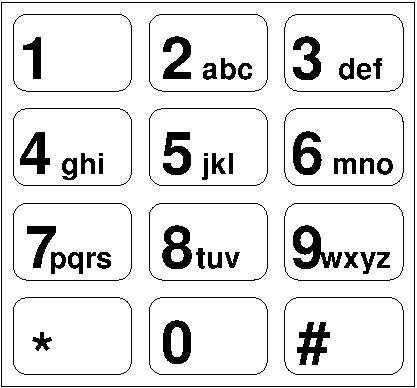
\includegraphics[width=1.8in]{finnish_mobile_phone_keypad.pdf}
\caption{The 12-key keypad of a typical Finnish mobile phone. There are three letters in the Finnish alphabet "\"{a}", "å" and "\"{o}", which are not shown on the keypad. The
  letters "\"{a}" and "å" are entered pressing key "2" four times and
  five times respectively. The letter "\"{o}" is entered by pressing
  the key "6" four times.}\label{keypad}
\end{center}
\end{figure}

Mobile phone text messages are a hugely popular means of
communication, but mobile phones are not especially well suited for
inputting text because of their small size and often limited
keyboard. There exist several technological solutions for inputting text
on mobile phones and other limited keyboard devices. This paper is
concerned with a technology called predictive text entry, which
utilizes redundancy in natural language in order to enable efficient
text entry using limited keyboards (typically having 12 keys).



The subject of predictive text entry has been extensively studied, but
the studies have mainly concerned on predictive text entry of
English. Because of the limited morphological complexity of English,
these approaches have usually been able to rely on an extensive
dictionary along with word frequencies, since a sufficiently large
English dictionary nearly eliminates the problem of out-of-vocabulary
words. 

For morphologically complex languages like Finnish or Turkish,
productive inflection, derivation and compounding raise the number of
out-of-vocabulary words regardless of the size of the dictionary,
which means that out-of-vocabulary words present a serious problem for
dictionary based approaches to predictive text entry.

In this paper we present an approach to predictive text entry which is
based upon a morphologically segmented training corpus and a
probabilistic model on phonotax. We additionally use a probabilistic
model on letter sequences and phonological rules governing the vowel
harmony phenomenon in Finnish. We show that this model delivers
superior results compared to an existing dictionary based model for
text entry of Finnish when evaluated on actual text-message data using
the keystroke per character ratio (KPC). We also compare our method to
the predictive text entry in three commercially available mobile
phones and show that our approach gives superior KPC.

Apart from phonological rules, our approach is entirely unsupervised
and data-driven, since we us the unsupervised morphological
segmentation system Morfessor \cite{Creutz07ACMTSLP} for segmenting
the training corpus and the tools for constructing POS-taggers form the HFST interface~\cite{hfst/2011}. We show that it can be applied to another
agglutinative language besides Finnish, namely Turkish. We compare the
Turkish text entry system to an existing text entry system, which is
based on a hidden Markov model and show that our approach gives a
substantial improvement in KPC.

The paper is structured as follows. In section~\ref{earlier-work} we
present some earlier approaches to predictive text entry. In
section~\ref{model}, we present our probabilistic model for text entry
together with the phonological rules which are used to realize vowel
harmony and explain how these models are combined into a system for
predictive text entry. Section~\ref{data} describes the training and
test corpora used in constructing and testing predictive text entry
systems for Finnish and Turkish. Evaluation of the systems is
presented in section~\ref{evaluation} and the results are discussed in
section~\ref{discussion}. Finally we present some concluding remarks
and future work directions in section~\ref{conclusion}.

\section{Earlier Approaches to Predictive Text Entry}\label{earlier-work}

Lore ipsum...

\section{A Probabilistic Model of Word Structure}\label{model}

Predictive text entry can be seen as a labeling task, where every key
in a sequence of keys is assigned its most likely letter. An obvious
approach to modeling such correspondences of keystroke sequences and
letters is using a stochastic model with hidden variables, such as a
hidden Markov model.

Though predictive text entry can be modeled fairly well using hidden
Markov models on key sequences as demonstrated by~\cite{Tantug:2010},
there are problems with this approach for agglutinative languages. A
second or third order HMM cannot encode very long dependencies inside
words. This leads to difficulties in processing agglutinative
languages, since it is difficult to separate stems from affixes in an
adequate manner and to handle arbitrarily long phonological
dependencies like vowel harmony in Finnish and Turkish. Using higher
order HMMs could in theory lead to better accuracy for longer
dependencies, but higher order HMMs suffer both from the data
sparseness problem and efficiency problems, which limit their
usability.

We observed earlier that dictionary based methods produce poor results
for agglutinative languages. Still the number of word stems seen in
training corpora of comparable sizes for agglutinative and isolating
languages are comparable. The reasons that make dictionary based
models fare poorly for agglutinative languages are thus inflection,
compounding and derivation. 

In order to get a general enough model of words and still be able to
model word structure at a global level, we model words as sequences of
morphs, which are extracted from an automatically segmented training
corpus. To illustrate our approach we need to look at some Finnish
training data. There will probably be some occurrences of the word
form "taloa" (sg. partitive case of the word house). Automatic
segmentation of the training corpus might give the segmentation "talo
+ a", where the stem "talo" and the ending "a" are segmented into
different morphs. If the word form "taloakin" (sg. partitive case of
the word house with the clitic "kin") doesn't occur in the training
data, we can still esitmate its probability by looking at how probable
the morph combinations "talo + a" and "a + kin" are in the training
corpus.

The model we have chosen is a Markov chain of morph sequences. A
Markov chain on morph sequences is likely to suffer from the data
sparseness problem especially when trying to estimate the probability
of word forms whose stem has occurred few times (perhaps only once) in
the training corpus. Also productive compounding presents a problem,
because there are infinitely many ways in which word stems can combine
to form new word forms. We therefore combine the Markov chain of morph
sequences with an HMM which maps key sequences to letter sequences.

For the Finnish example in the previous paragraph, the HMM gives an
estimate for the probability of the sequence of letters "t-a-l-o",
given the input key-sequence "8-2-5-6". The HMM doesn't include
morph boundaries, so it gives some estimate for the probability of
the wordform "a-l-a-t-a-l-o" (a common Finnish surname) given its keystring
"2-5-2-8-2-5-6", even though the combination of morphs "ala + talo"
would never have been observed in the training data and the morph
sequence model would therefore be unable to give a good estimate for
the probability of the compound word.

Finally many agglutinative languages like Finnish and Turkish
incorporate phonological phenomena, such as vowel harmony, which span
over entire word forms consisting of several morphs. E.g. the Finnish
inessive case ending is "ssA", where "A" is either "a" or "\"{a}"
depending on whether the stem of the wordform has front vowels "ä",
"ö", "y" or back vowels "a", "o", "u" (usually front vowels and back
vowels cannot be mixed). Since "a" and "\"{a}" are typed using the
same key "2", the vowel is always ambiguous in the ending. Consider
the segmented form "talo + i + ssa" (pl. inessive case of the word
house), the final is "a" which can be deduced from the vowel "o" in
the stem, but neither the morph sequence model nor the letter HMM can
disambiguate between "a" and "ä". The morpheme sequence model doesn't
aid in disambiguation, since it looks at adjacent morphs and the stem
and ending "ss\"{a}" are separated by the plural morph "i". Also the
letter sequence HMM fails to disambiguate between the front and back
vowel, since it can only consider the co-occurrence of letters that
are separated by less than three letters and the letters "o" and "a"
in the word form "taloissa" are separated by exactly three letters
(including "a" and "o").

Using a second order morph sequence model, might possibly handle some
cases of vowel harmony, but data sparseness is a serious problem with
the morph sequence model, since there are tens of thousands of
distinct morphs. Therefore long range phenomena like vowel harmony
cannot be adequately captured using n-gram models of morphs or
letters, which has prompted us to use phonological rules which realize
the constraints as part of our system.

The statistical models and phonological rules are implemented as
weighted finite-state transducers, which allows combining them using
the algebraic operations for finite-state transducers. Transducers are
a natural choice for coding arbitrarily long dependencies such as
vowel harmony, which cannot be captured by Markov models.

\subsection{A Hidden Markov Model for Predicting Letter Sequences from Key Sequences}

We denote a sequence of mobile phone keypad keys of length $n$ by $K =
(k_i)_{i=1}^{n}$. Here each $k_i$ corresponds to a key on the mobile
phone keypad. For the key $k$, we denote the set of letters
corresponding to the key $k$ by ${\rm M}(k)$. E.g. ${\rm M}(2) = \{$
a, b, c, \"{a}$\}$ on a typical Finnish mobile phone
keyboard. Correspondingly, we denote a sequences of letter of length
$m$ by $L = (l_i)_{i=1}^{m}$.

The task in the letter model is to give the probability of a letter
sequence $L$ given a sequence of keys $K$. Naturally ${\rm P}(L|K) > 0$, iff
$L \in {\rm M}(K)$. The probability ${\rm P}(L|K)$ is given in equation (\ref{letter-chain-eqn}).  


\subsection{A Markov Chain of Morphs}

A morph of $n$ letters in the training-data is just a sequence of $n$
letters, so we denote it by $L = (l_i)_{i=1}^{n}$. A key sequence $K =
(k_i)_{i=1}^{m}$ corresponds to a sequence of morphs $L_1{\rm
  ... }L_k$ , where each $L_j = (l_{j_i})_{i=1}^{n_j}$, iff $\Sigma_{j
  = 1}^{k} n_j = m$ and $l_{j_i} \in {\rm M}(k_{m_1 + {\rm ... } +
  m_{j - 1} + i})$ for all $l_{j_i}$. We denote the set of morph
sequences that correspond to a key sequence $K$ by ${\rm M}(K)$.

The task of the morph model is to assign a probability for each
sequence of morphs in ${\rm M}(K)$ for a key sequence $K$. The
probability of a sequence of morphs $L_1{\rm ... }L_k \in {\rm M}(K)$
is given by the chain rule of probabilities in equation
(\ref{chain-eqn}).
\begin{equation}\label{chain-eqn}
{\rm P}\big(L_1{\rm, ..., }\ L_k\big) = {\rm P}(L_1 | L_2 {\rm, ..., }\ L_k) {\rm P}(L_2 | L_3 {\rm, ..., }\ L_k)\ {\rm ... }\ {\rm P}(L_{k-1} | L_k){\rm P}(L_k)
\end{equation}

We make the standard assumptions for a first order Markov model and approximate equation (\ref{chain-eqn}) by equation (\ref{markov-eqn}).
\begin{equation}\label{markov-eqn}
{\rm P}\big(L_1{\rm, ..., }L_k\big) = {\rm P}\big(L_1 | L_2){\rm P}\big(L_2 | L_3)\ {\rm ... }\ {\rm P}(L_{k-1} | L_k){\rm P}(L_k)
\end{equation}

It should be noted that we are dealing with morph sequences and not
letter strings. This is important, since several morph sequences can
correspond to the same string of letters.

\subsection{Phonological Constraints}

\subsection{Combining Models using Weighted Finite-State Calculus}

\section{Training Materials and Test Materials for Finnish and Turkish}\label{data}

\subsection{Finnish}

For training and testing the Finnish text entry system, we use the
same data as \cite{silfverberg/2011/cla}, though they use a
morphological analyzer, which we do not utilize. The training material is extracted from Finnish IRC logs and contains some 350000 words. The test material is actual text message data and contains $6663$ words~\footnote{The original test data contains $10851$ words, but it turned out that the latter part of the test data file is actually a list of unique words, which would skew test results, so we decided to only use the earlier half of the material}. 

\subsection{Turkish}

For training and testing the Turkish text entry system, we use the
same materials as \cite{Tantug:2010}. The material is divided into a
test corpus containing $2597$ words and a training corpus which
includes the rest of the words in the material. Thus the training data
and test data are disjoint.

\section{Evaluation}\label{evaluation}

In this section, we present the results of experiments using the
Finnish and Turkish training data and test data presented in the
previous section. For Finnish we examine the impact of varying the
amount of training data on the performance of the predictive text
entry system. For Turkish we present results on the whole test
material.

\subsection{The Keystrokes Per Characters Ratio}

Many factors influence the efficiency of mobile phone text entry in
practice. E.g. the general user interface design of the phone and
specifically the design of the keyboard have a large
impact. Nevertheless such factors are in some sense isolated from the
predictive text entry algorithm itself, which makes it plausible to
evaluate the algorithms in isolation from the rest of the user
interface of mobile phones. In this paper we use the keystrokes per
character (KPC) ratio~\cite{MacKenzie02kspc} for measuring the
efficiency of text entry. It measures the average number of keystrokes
required to input one letter in a text message. As a measure of the
efficiency of predictive text input, keystrokes per character leaves
something to be desired, since it in no way incorporates factors such
as cognitive workload, but such factors could not be adequately
addressed in a paper on computational linguistics. Moreover they
cannot be studied in isolation from the user interface of the mobile
phone.

The keystroke per character ratio is computed on test data as the
ratio of keystrokes used to enter the data using a given text entry
method and the number of letters in the words in the data. Following
\cite{Tantug:2010}, we do not consider space characters as a part of
the test data.

For the multitap method inputting the Finnish word "kukka" (flower) on
a typical Finnish 12-key mobile phone keyboard requires 10 keystrokes
as shown in figure~\ref{kukka-kpc}. Hence the KPC ratio for test data
consisting of the single word "kukka" would be $10/5 = 2.0$.

For our own method we compute KPC similarly as for multitap, by
dividing the number of keystrokes used by the number of letters in the
test data. If our method cannot provide the correct suggestion for
some input sequence, we use multitap as a fallback method. Naturally
we cannot know that a word is not given by the text entry method
before scrolling through all of the suggestions, so entering an
unknown word requires:
\begin{enumerate}
\item Entering the keys used to write the word (one keystroke per letter)
\item Scrolling through the suggestions ($9$ keystrokes in the current system, since there are $10$ suggestions)
\item Deleting the last suggestion one letter at a time (one keystroke per letter)
\item Switching to multitap mode (one keystroke)
\item Inputting the word in multitap mode (keystroke count varies depending on the word).
\end{enumerate}

Figure \ref{new-method-kpc-known} demonstrates how KPC is computed for
entering the word "\"{o}it\"{a}" (nights) using our own text entry
method. The figure \ref{new-method-kpc-unknown} shows inputting the word "subi" (probably a
Finnish version of sub). The correct form of "subi" is not found using our text
entry method, which means we need to use multitap as fallback.

\begin{figure}[htb!]
\begin{center}
\begin{tabular}{llllll}
\texttt{k} & \texttt{u} & \texttt{k} & & \texttt{k} & \texttt{a}
\\ \texttt{5-5} & \texttt{8-8} & \texttt{5-5} & \texttt{<NEXT>} &
\texttt{5-5} & \texttt{2}
\end{tabular}
\caption{Inputting the Finnish word "kukka" using the multitap method
  for text entry requires $10$ keystrokes. Pressing the
  \texttt{<NEXT>} key is required, since there are two consecutive
  letters "k" in "kukka".}\label{kukka-kpc}
\end{center}
\end{figure}

\begin{figure}[htb!]
\begin{center}
\begin{tabular}{lllllllllllllllllllll}
\texttt{\"{m}} & \texttt{i} & \texttt{t} & \texttt{\"{a}} & \\ 
\texttt{\"{o}} & \texttt{i} & \texttt{t} & \texttt{\"{a}} & \\ 
\texttt{6} & \texttt{4} & \texttt{8} & \texttt{2} & \texttt{<NEXT>}\\\\
\end{tabular}
\end{center}
\caption{Inputting the Finnish words "\"{o}it\"{a}" and "subi". The first suggestion for the input sequence \texttt{6-4-8-2} is "mit\"{a}" (what). Hence we need to press \texttt{<NEXT>} once to reach the second suggestion which is correct. All in all, this makes \texttt{4 + 1 = 5} keystrokes.} \label{new-method-kpc-known}
\end{figure}

\begin{figure}[htb!]
\begin{center}
\begin{tabular}{lllllllllllllllllllll}
\texttt{s} & \texttt{u} & \texttt{c} & \texttt{h}\\
...\\
\texttt{s} & \texttt{t} & \texttt{a} & \texttt{h}\\
\texttt{s} & \texttt{u} & \texttt{b} & \texttt{i}\\    
\texttt{7} & \texttt{8} & \texttt{2} & \texttt{4} & \texttt{<NEXT>} & \texttt{...} & \texttt{<NEXT>} & \texttt{<C>} & \texttt{<C>} & \texttt{<C>} & \texttt{<C>} & \texttt{<MUL>} & \texttt{7-7-7-7} & \texttt{8-8} & \texttt{2-2} & \texttt{4-4-4} & \texttt{<PRED>}
\end{tabular}

\caption{The word "subi" is not given by our method, so we need to scroll through ten suggestions using \texttt{<NEXT>} nine times, then delete the letters in the last suggestion "stah", switch to multitap mode using the key \texttt{<MUL>}, input "subi" in multitap and switch back to predictive mode using the key \texttt{<PRED>}. Thus inputting "subi" requires $4 + 9 + 4 + 1 + 11 + 1 = 30$ keystrokes.} \label{new-method-kpc-unknown}
\end{center}
\end{figure}



\begin{figure}[hbt!]
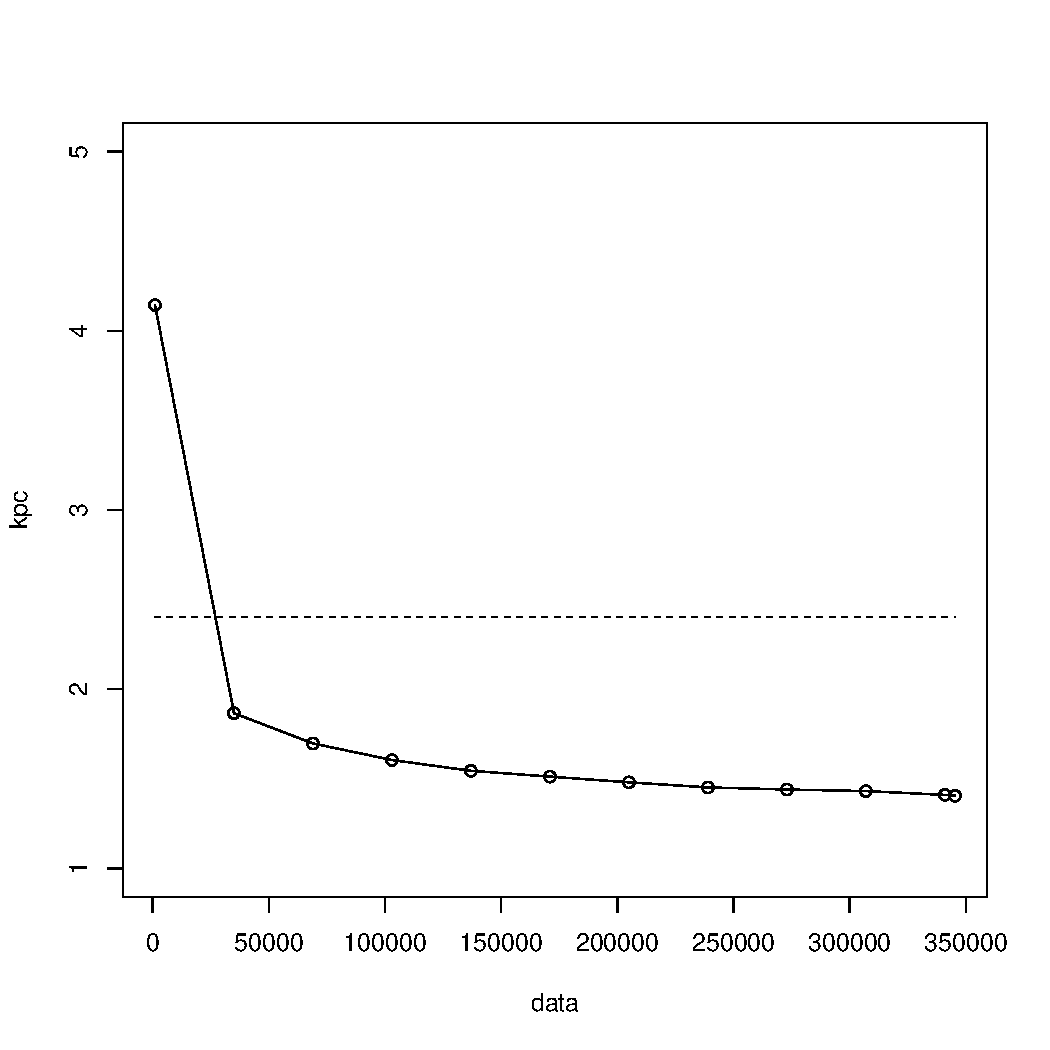
\includegraphics[width=4in]{finnish_kpc_figure.pdf}
\end{figure}

\section{Discussion}\label{discussion}

\section{Conclusions and future work}\label{conclusion}

\section{Acknowledgments}

\bibliographystyle{splncs03}
\bibliography{cicling2011.bib}
\end{document}
